\chapter{Oracle Aplication Express}

\section{Cara Membuat Aplikasi Pada Oracle Apex}

\begin{enumerate}





\begin{figure}[!htbp]
\item[1] Pilih "App Builder".
    \begin{center}
    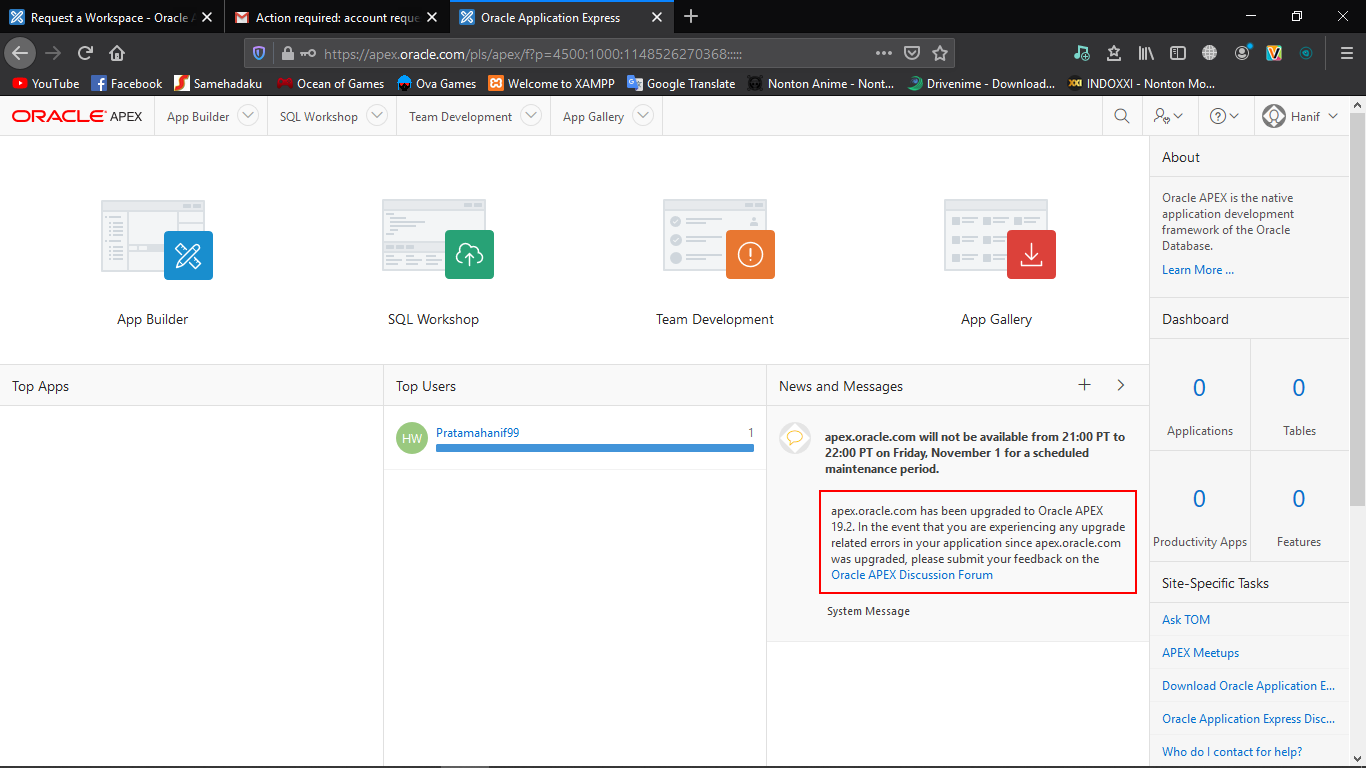
\includegraphics[scale=0.3]{section/Screenshot(28).png}
    \end{center}
    \end{figure}
    
\begin{figure}[!htbp]
\item[2] Pilih "Create".
\begin{center}
    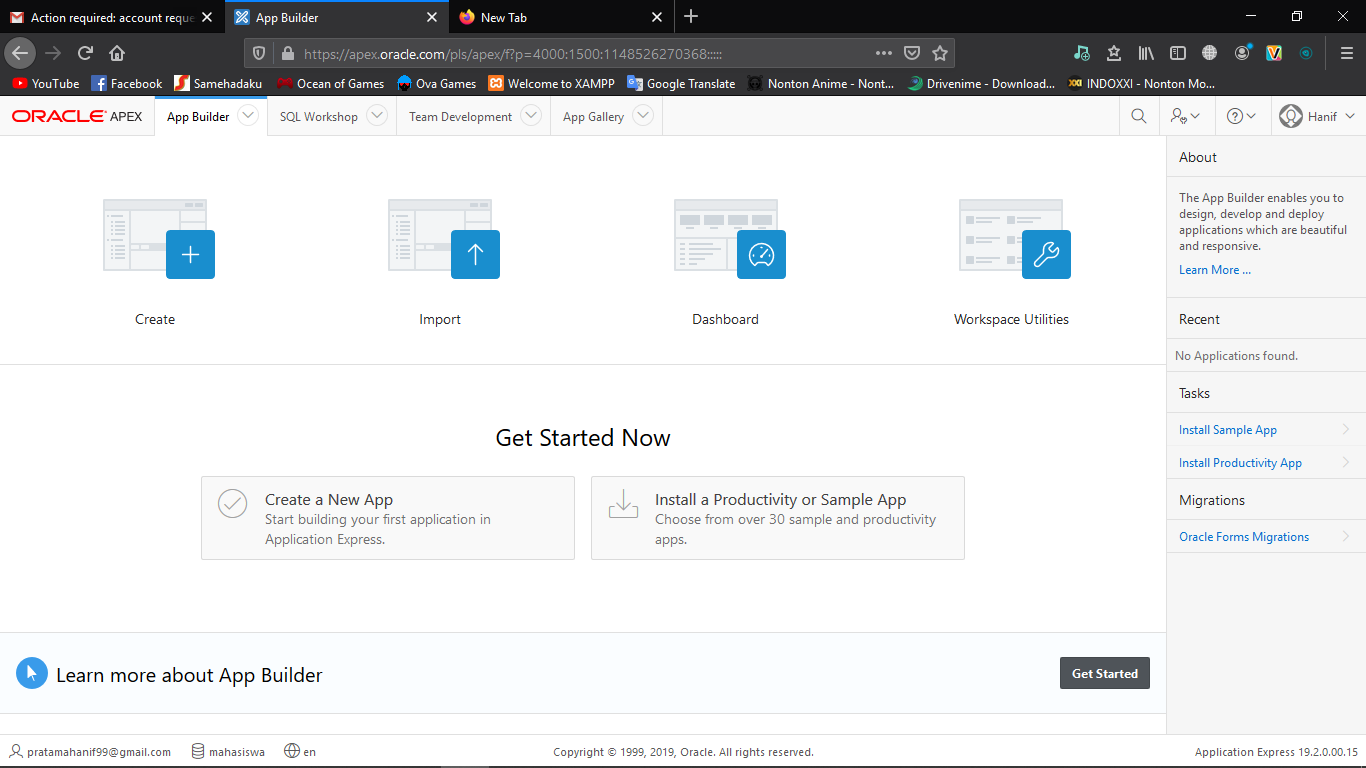
\includegraphics[scale=0.3]{section/Screenshot(29).png}
    \end{center}
    \end{figure}
    
\begin{figure}[!htbp]    
\item[3] Klik from a file.
\begin{center}
    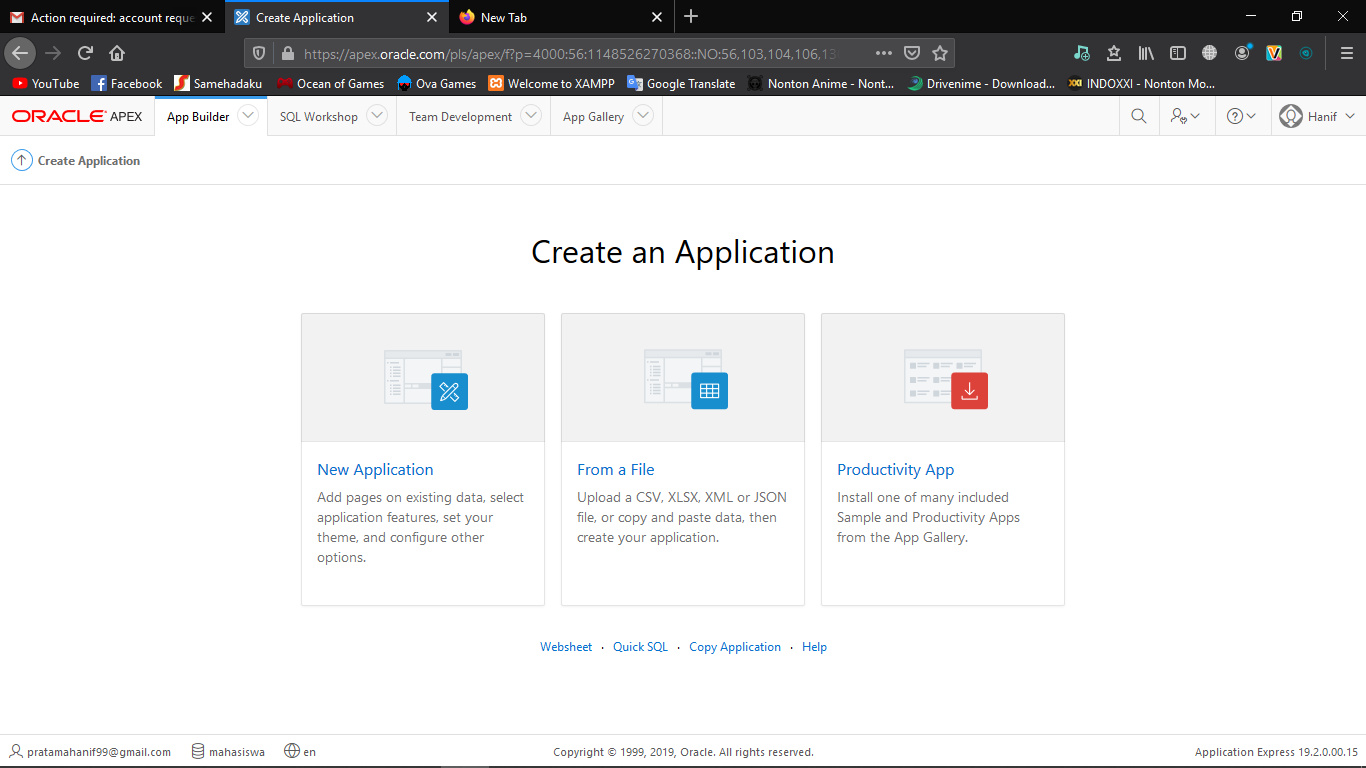
\includegraphics[scale=0.3]{section/Screenshot(30).png}
    \end{center}
    \end{figure}

\begin{figure}[!htbp]
\item[4] Pilih file yang akan dipilih.
\begin{center}
    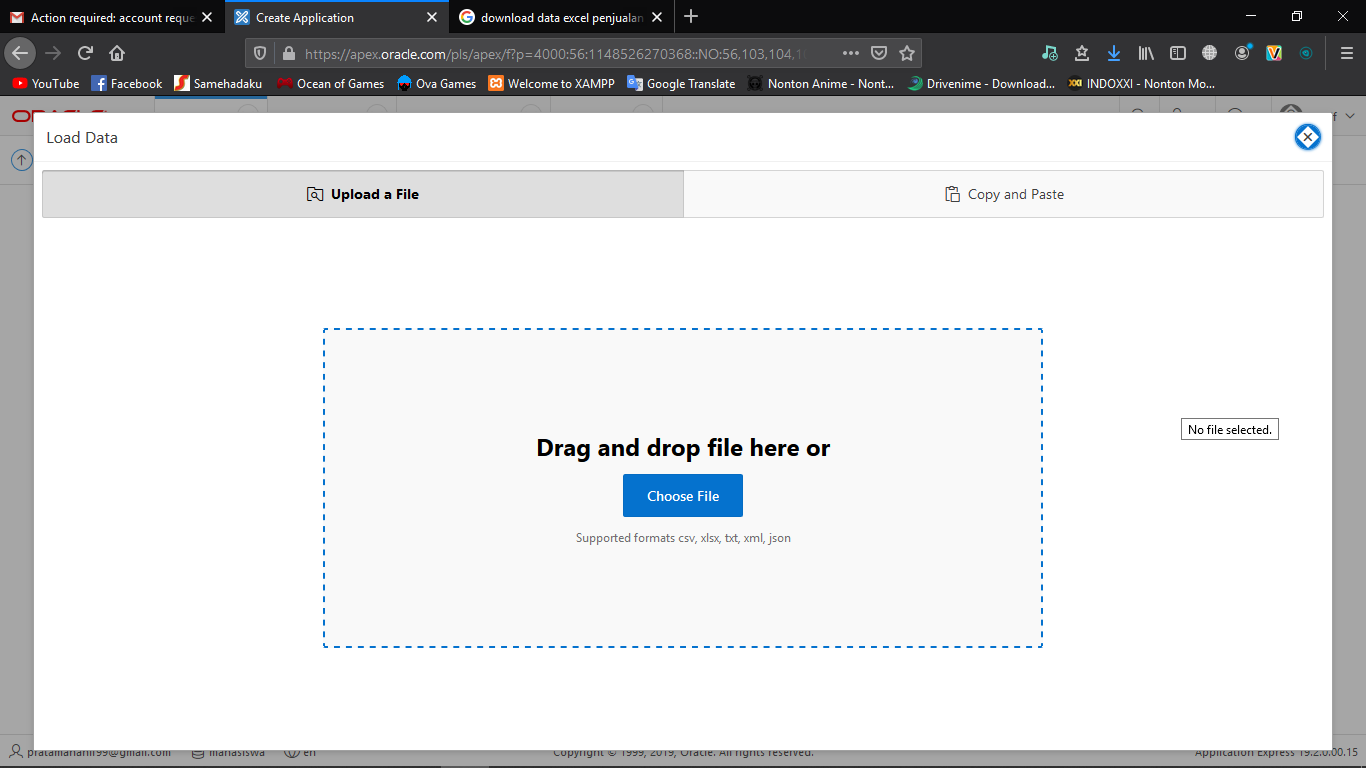
\includegraphics[scale=0.3]{section/Screenshot(31).png}
    \end{center}
    \end{figure}

\begin{figure}[!htbp]    
\item[5] Klik file yang akan dipilih.
\begin{center}
    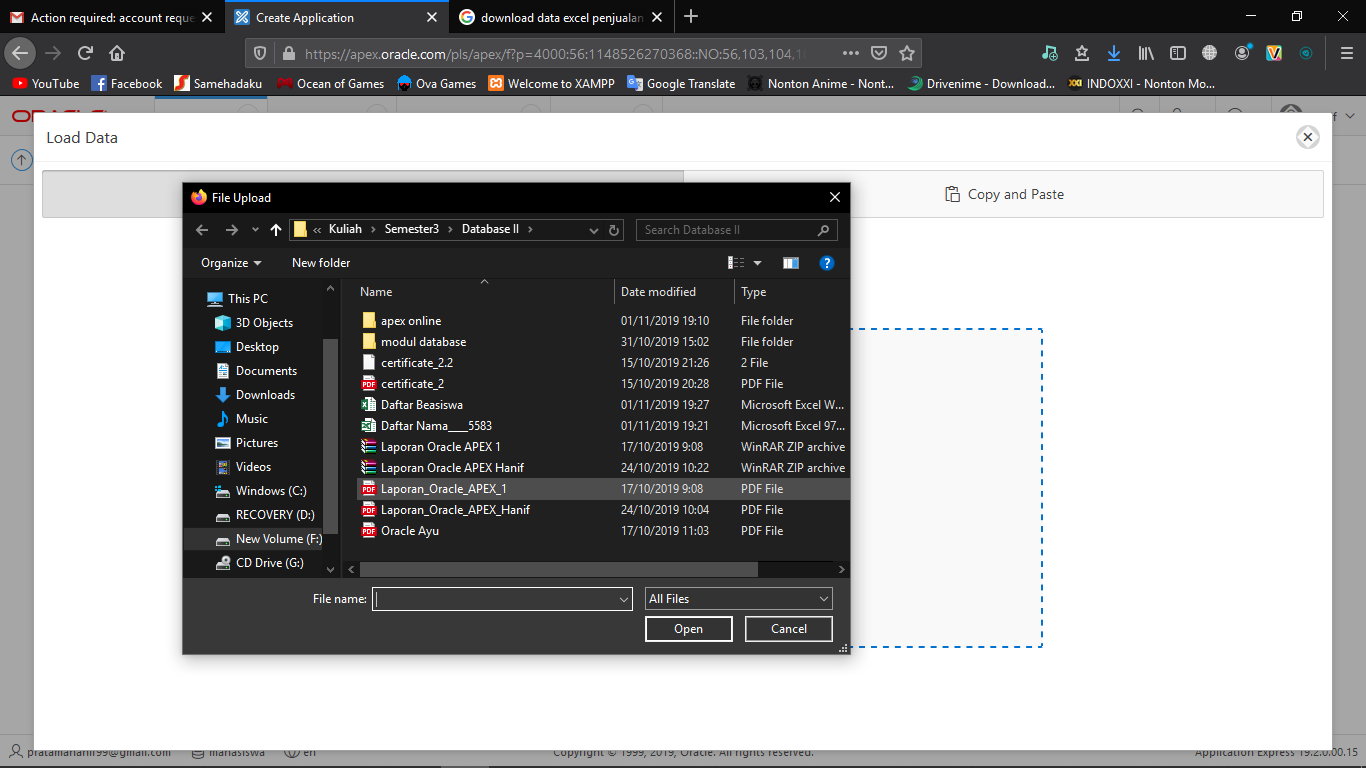
\includegraphics[scale=0.3]{section/Screenshot(32).png}
    \end{center}
    \end{figure}
    
\begin{figure}[!htbp]
\item[6] Isi table  name, klik load data
\begin{center}
    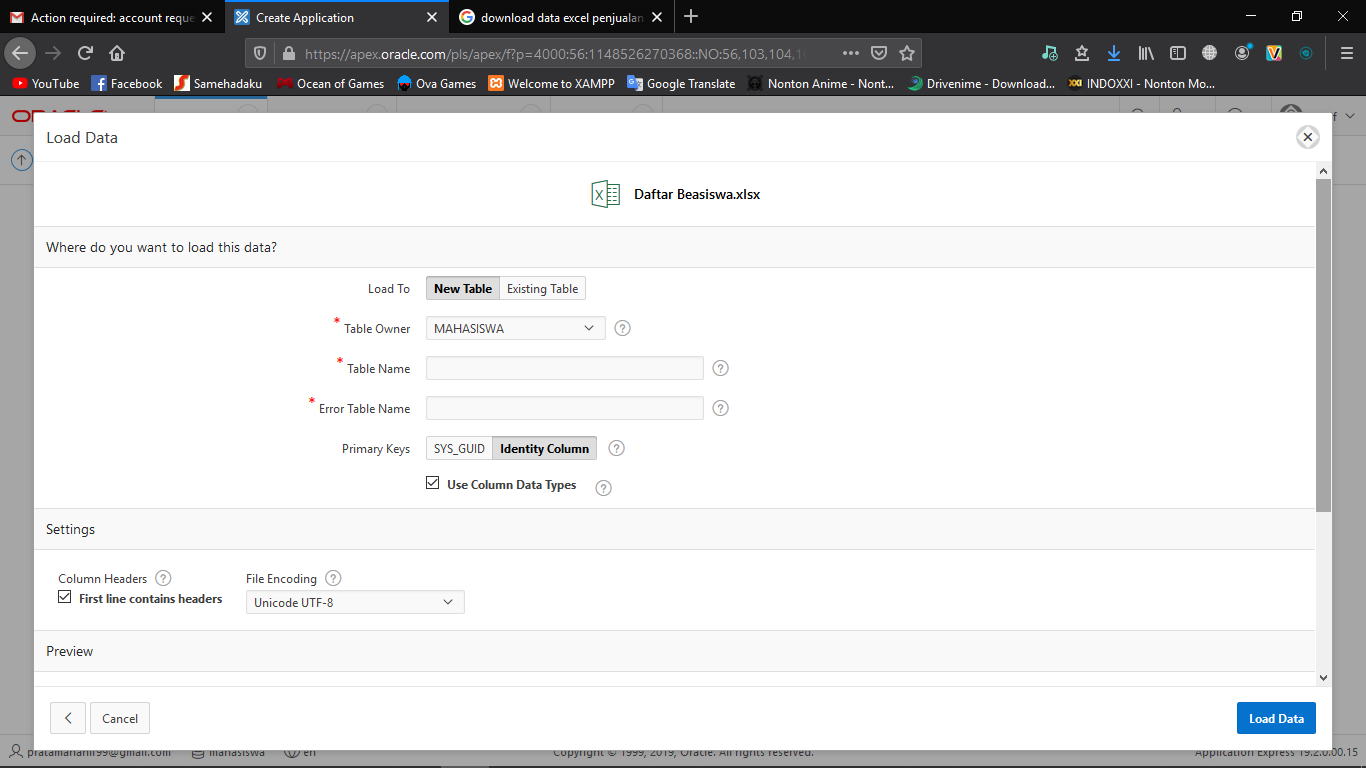
\includegraphics[scale=0.3]{section/Screenshot(33).png}
    \end{center}
    \end{figure}
    
\begin{figure}[!htbp]    
\item[7] Table sudah dibuat
\begin{center}
    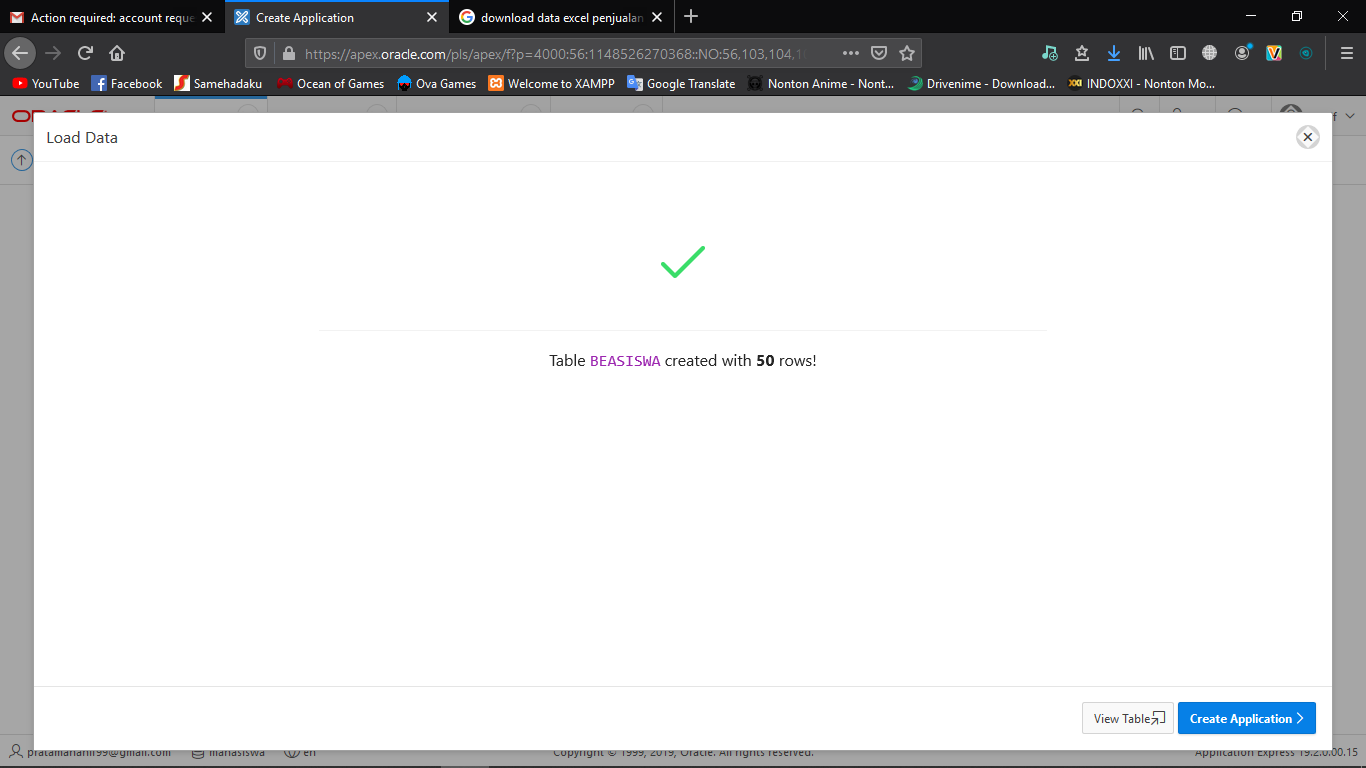
\includegraphics[scale=0.3]{section/Screenshot(34).png}
    \end{center}
    \end{figure}
    
\begin{figure}[!htbp]
\item[8] Scroll ke bawah, klik create application
\begin{center}
    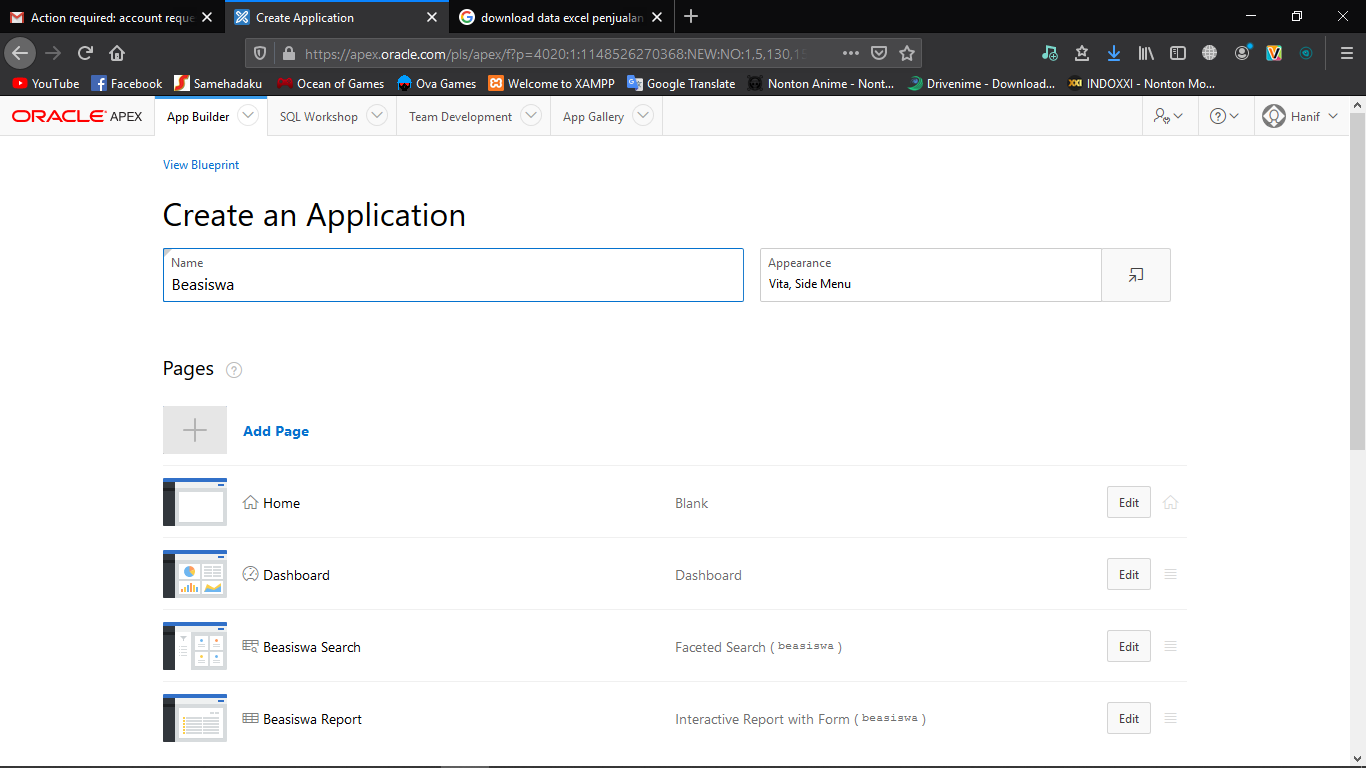
\includegraphics[scale=0.3]{section/Screenshot(35).png}
    \end{center}
    \end{figure}
    
\begin{figure}[!htbp]
\item[9] Pilih run  application
\begin{center}
    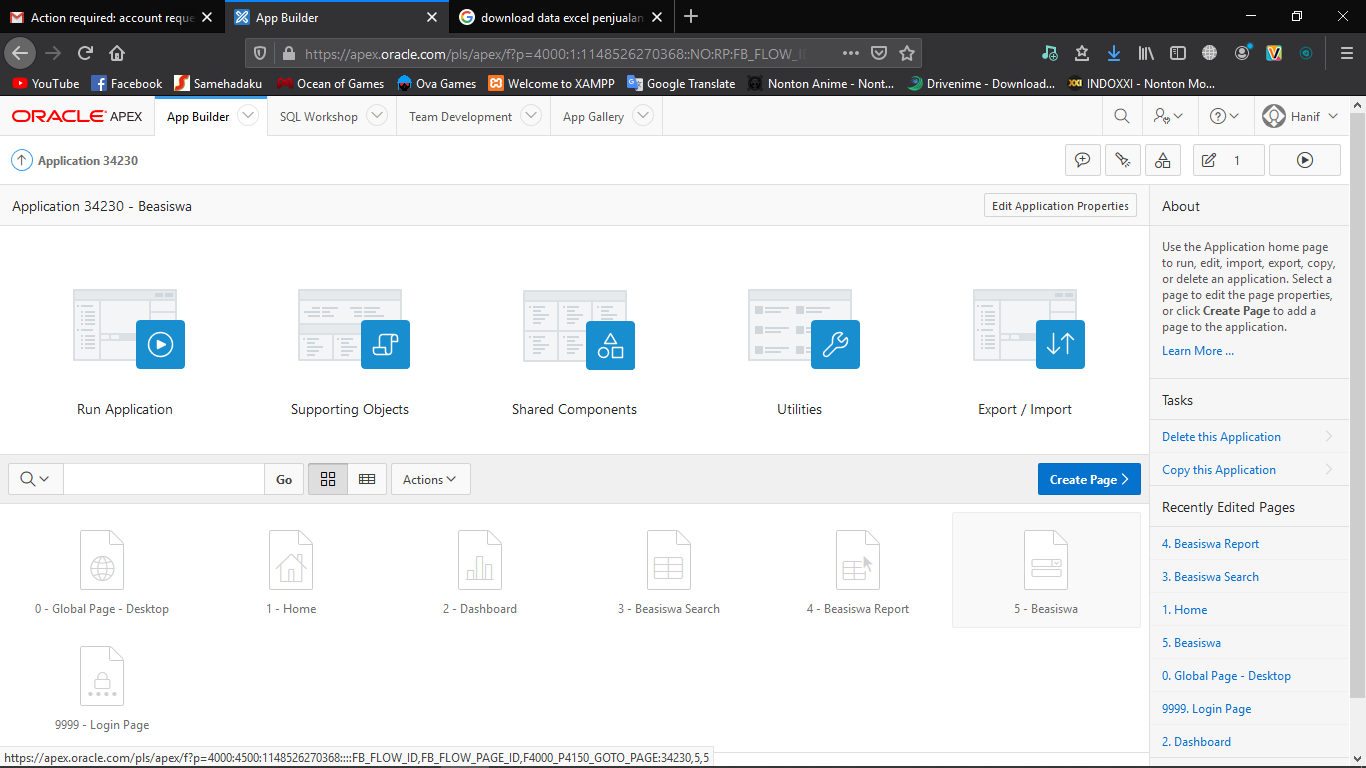
\includegraphics[scale=0.3]{section/Screenshot(36).png}
    \end{center}
    \end{figure}
    
\begin{figure}[!htbp]
\item[10] Login dengan akun yang sudah dibuat
\begin{center}
    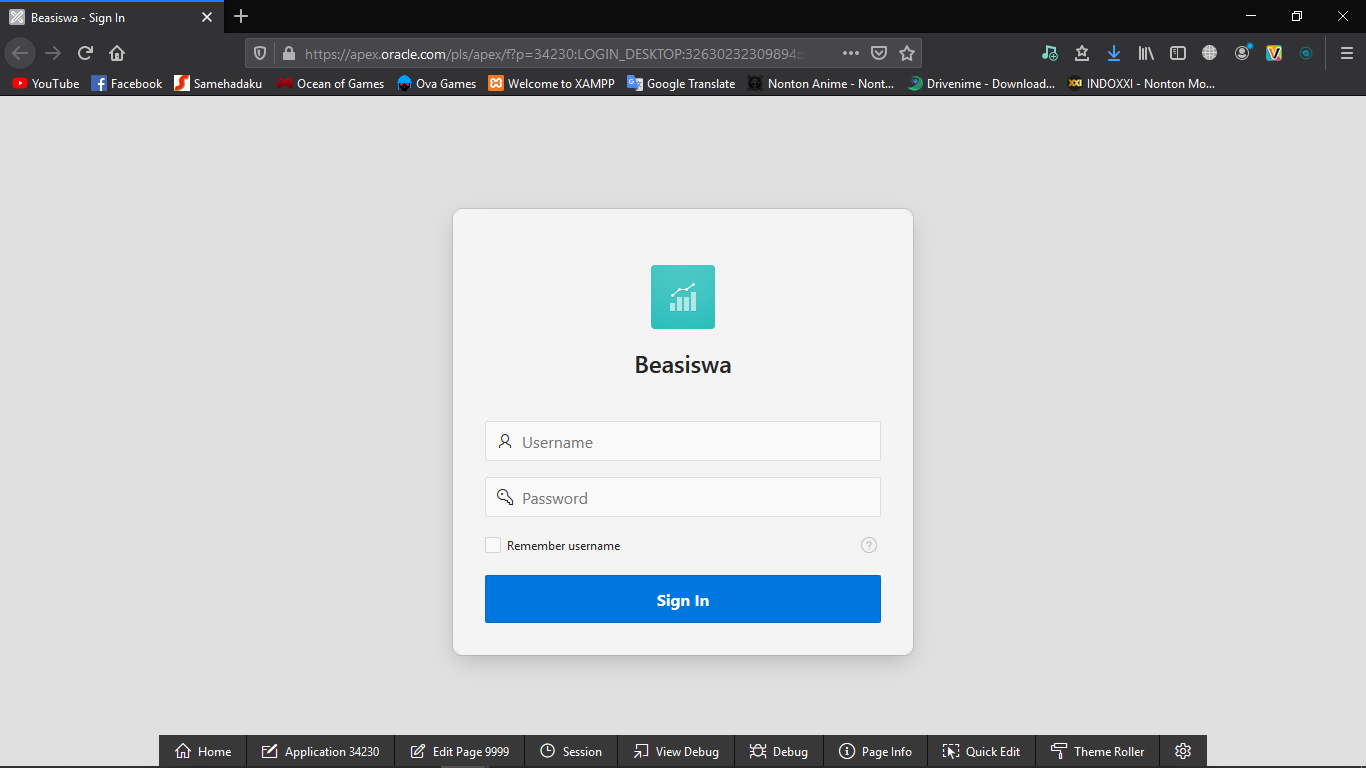
\includegraphics[scale=0.3]{section/Screenshot(37).png}
    \end{center}
    \end{figure}
    
\begin{figure}[!htbp]
\item[11] Aplikasi siap digunakan, untuk melihat data, pilih beasiswa report. Untuk membuka aplikasi di perangakt lain, buka link URL-nya yaitu
 https://apex.oracle.com/pls/apex/f?p=34230:LOGIN\_DESKTOP:103665404926840:::::
\begin{center}
    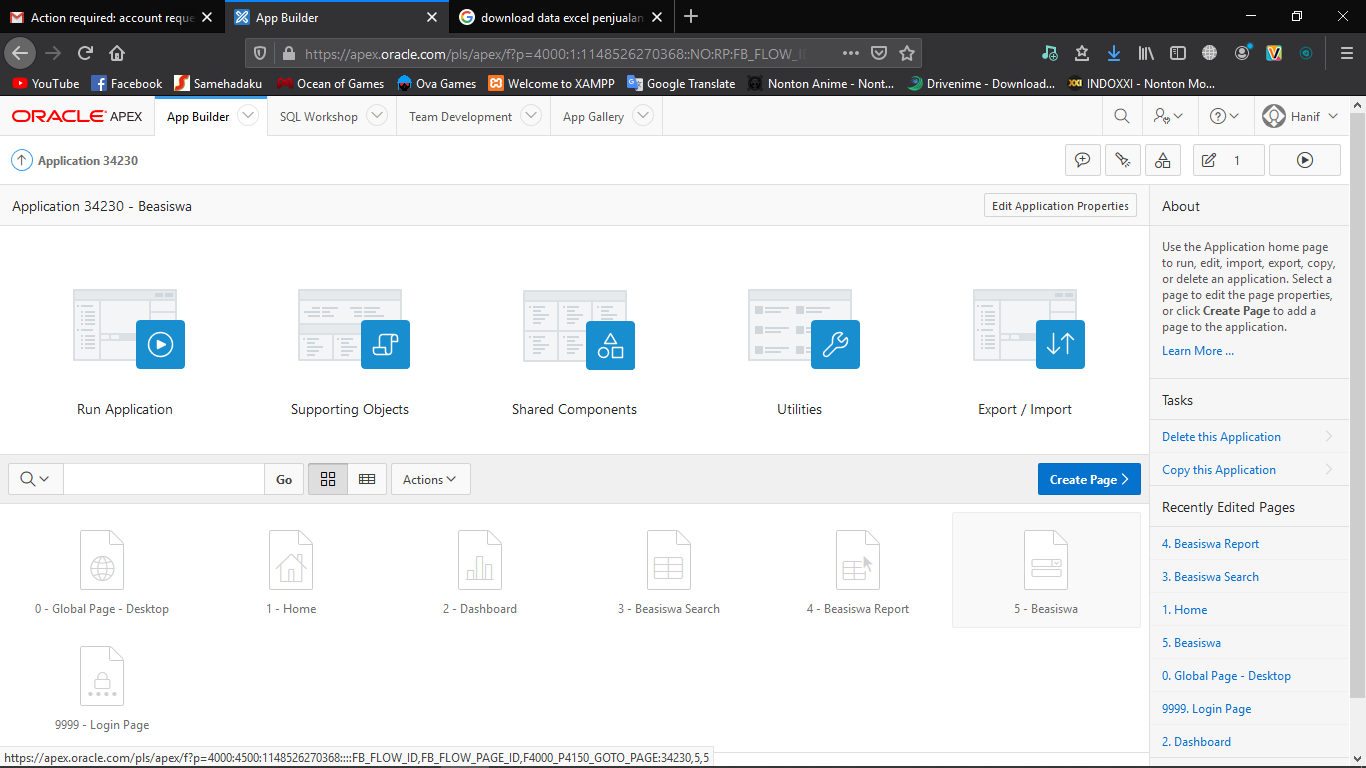
\includegraphics[scale=0.3]{section/Screenshot(36).png}
    \end{center}
    \end{figure}    
\end{enumerate}


